%input macros (i.e. write your own macros file called MacroFile1.tex)
%\newcommand{\PdfPsText}[2]{
  \ifpdf
     #1
  \else
     #2
  \fi
}

\newcommand{\IncludeGraphicsH}[3]{
  \PdfPsText{\includegraphics[height=#2]{#1}}{\includegraphics[bb = #3, height=#2]{#1}}
}

\newcommand{\IncludeGraphicsW}[3]{
  \PdfPsText{\includegraphics[width=#2]{#1}}{\includegraphics[bb = #3, width=#2]{#1}}
}

\newcommand{\InsertFig}[3]{
  \begin{figure}[!htbp]
    \begin{center}
      \leavevmode
      #1
      \caption{#2}
      \label{#3}
    \end{center}
  \end{figure}
}


%%% Local Variables: 
%%% mode: latex
%%% TeX-master: "~/Documents/LaTeX/CUEDThesisPSnPDF/thesis"
%%% End: 


 \documentclass[oneside,12pt]{Classes/CUEDthesisPSnPDF}


\ifpdf
    \pdfinfo { /Title  (CUED PhD and MPhil Thesis Classes)
               /Creator (TeX)
               /Producer (pdfTeX)
               /Author (Harish Bhanderi harish.bhanderi@cantab.net)
               /CreationDate (D:20030101000000)  %format D:YYYYMMDDhhmmss
               /ModDate (D:20030815213532)
               /Subject (Writing a PhD thesis in LaTeX)
               /Keywords (PhD, Thesis)}
    \pdfcatalog { /PageMode (/UseOutlines)
                  /OpenAction (fitbh)  }
\fi

\title{Writing a PhD Thesis\\[1ex]
        in \LaTeXe}

\ifpdf
  \author{\href{mailto:harish.bhanderi@cantab.net}{Harish Bhanderi}}
  \collegeordept{\href{http://www.eng.cam.ac.uk}{Department of Engineering}}
  \university{\href{http://www.cam.ac.uk}{University of Cambridge}}
% insert below the file name that contains the crest in-place of 'UnivShield'
  \crest{
\includegraphics[width=30mm]{UnivShield}}
\else
  \author{Harish Bhanderi}
  \collegeordept{Department of Engineering}
  \university{University of Cambridge}
% insert below the file name that contains the crest in-place of 'UnivShield'
  \crest{
\includegraphics[bb = 0 0 292 336, width=30mm]{UnivShield}}
\fi
%
% insert below the file name that contains the crest in-place of 'UnivShield'
% \crest{\IncludeGraphicsW{UnivShield}{40mm}{14 14 73 81}}
%
%\renewcommand{\submittedtext}{change the default text here if needed}
\degree{Doctor of Philosophy}
\degreedate{Yet to be decided}

% turn of those nasty overfull and underfull hboxes
\hbadness=10000
\hfuzz=50pt

% Put all the style files you want in the directory StyleFiles and usepackage like this:
\usepackage{StyleFiles/watermark}

% Comment out the next line to get single spacing
\onehalfspacing

\begin{document}

%\language{english}

% A page with the abstract on including title and author etc may be
% required to be handed in separately. If this is not so, then comment
% the below 3 lines (between '\begin{abstractseparte}' and 
% 'end{abstractseparate}'), normally like a declaration ... needs some more
% work, mind as environment abstracts creates a new page!
% \begin{abstractseparate}
%   %!TEX root = thesis.tex

Three Dimensional (3D) palmprint has proved to be a significant biometrics for personal authentication. 3D palmprints are harder to counterfeit than 2D palmprints and more robust to variations in illumination and serious scrabbling on the palm surface. Previous work on 3D palmprint recognition has concentrated on local features such as texture and lines.

% a blank line as required
\vspace{12pt}

In this dissertation, the authentication process are improved using 3D features. The features are stable in samples from a single person over time and distinguishable among samples from different people. Three features adopted are Maximum Depth of palm center, Horizontal Cross-section Area and Radial Line Length from the centroid to the boundary of 3D palmprint horizontal cross-section of different levels. The feature set is combined as a column feature vector for matching. Support Vector Machine is introduced for higher efficiency.

% a blank line as required
\vspace{12pt}

Experiments are conducted on an existing 3D palmprint database of 8,000 samples. The results show that the proposed method is able to achieve an reasonable performance.


% \textbf{Keywords}: 3D palmprint identification, 3D palmprint verification, SVM

% \end{abstractseparate}




% Using the watermark package which is in StyleFiles/
% and to remove DRAFT COPY ONLY appearing on the top of all pages comment out below line
%\watermark{DRAFT COPY ONLY}


\maketitle

%set the number of sectioning levels that get number and appear in the contents
\setcounter{secnumdepth}{3}
\setcounter{tocdepth}{3}

\frontmatter % book mode only
\pagenumbering{roman}
% Thesis Dedictation ---------------------------------------------------

\begin{dedication} %this creates the heading for the dedication page

I would like to dedicate this thesis to my loving parents ...

\end{dedication}

% ----------------------------------------------------------------------

%%% Local Variables: 
%%% mode: latex
%%% TeX-master: "../thesis"
%%% End: 

% Thesis Acknowledgements ------------------------------------------------


%\begin{acknowledgementslong} %uncommenting this line, gives a different acknowledgements heading
\begin{acknowledgements}      %this creates the heading for the acknowlegments


And I would like to acknowledge ...


\end{acknowledgements}
%\end{acknowledgmentslong}

% ------------------------------------------------------------------------

%%% Local Variables: 
%%% mode: latex
%%% TeX-master: "../thesis"
%%% End: 

%!TEX root = thesis.tex

Three Dimensional (3D) palmprint has proved to be a significant biometrics for personal authentication. 3D palmprints are harder to counterfeit than 2D palmprints and more robust to variations in illumination and serious scrabbling on the palm surface. Previous work on 3D palmprint recognition has concentrated on local features such as texture and lines.

% a blank line as required
\vspace{12pt}

In this dissertation, the authentication process are improved using 3D features. The features are stable in samples from a single person over time and distinguishable among samples from different people. Three features adopted are Maximum Depth of palm center, Horizontal Cross-section Area and Radial Line Length from the centroid to the boundary of 3D palmprint horizontal cross-section of different levels. The feature set is combined as a column feature vector for matching. Support Vector Machine is introduced for higher efficiency.

% a blank line as required
\vspace{12pt}

Experiments are conducted on an existing 3D palmprint database of 8,000 samples. The results show that the proposed method is able to achieve an reasonable performance.


% \textbf{Keywords}: 3D palmprint identification, 3D palmprint verification, SVM


\tableofcontents
\listoffigures
\printnomenclature  %% Print the nomenclature
\addcontentsline{toc}{chapter}{Nomenclature}

\mainmatter % book mode only
%%% Thesis Introduction --------------------------------------------------
\chapter{Introduction}
\ifpdf
    \graphicspath{{Introduction/IntroductionFigs/PNG/}{Introduction/IntroductionFigs/PDF/}{Introduction/IntroductionFigs/}}
\else
    \graphicspath{{Introduction/IntroductionFigs/EPS/}{Introduction/IntroductionFigs/}}
\fi

And this is how I would like to introduce my piece of work ...


blah blah blah blah blah blah blah blah blah blah blah blah blah blah blah blah blah blah blah blah blah blah blah blah blah blah blah blah blah blah blah blah blah blah blah blah blah blah blah blah blah blah blah blah blah blah blah blah blah blah blah blah blah blah blah blah blah blah blah blah blah blah blah blah blah blah blah blah blah blah blah blah blah blah blah blah blah blah blah blah blah blah blah blah blah blah blah blah blah blah blah blah blah blah blah blah blah blah blah blah blah blah blah blah blah blah blah blah blah blah blah blah blah blah blah blah blah blah blah blah blah blah blah blah blah blah blah blah blah blah blah blah blah blah blah blah blah blah blah blah blah blah blah blah blah blah blah blah blah blah blah blah blah blah blah blah blah blah blah blah blah blah blah blah blah blah blah blah blah blah blah blah blah blah blah blah blah blah blah blah blah blah blah blah blah blah blah blah blah blah blah blah blah blah blah blah blah blah blah blah blah blah blah blah blah blah blah blah blah blah blah blah blah blah blah blah blah blah blah blah blah blah blah blah blah blah blah blah blah blah blah blah blah blah blah blah blah blah blah blah blah blah blah blah blah blah blah blah blah blah blah blah blah blah blah blah blah blah blah blah blah blah blah blah blah blah blah blah blah blah blah blah blah blah blah blah blah blah blah blah blah blah blah blah blah blah blah blah blah blah blah blah blah blah blah blah blah blah blah blah blah blah blah blah blah blah blah blah blah blah blah blah blah blah blah blah blah blah blah blah blah blah blah blah blah blah blah blah blah blah blah blah blah blah blah blah blah blah blah blah blah blah blah blah blah blah blah blah blah blah blah blah blah blah blah blah blah blah blah blah blah blah blah blah blah blah blah blah blah blah blah blah blah blah blah blah blah blah blah blah blah blah blah blah blah blah blah blah blah blah blah blah blah blah blah blah blah blah blah blah blah blah blah blah blah blah blah blah blah blah blah blah blah blah blah blah blah blah blah blah blah blah blah blah blah blah blah blah blah blah blah blah blah blah blah blah blah blah blah blah blah blah blah blah blah blah blah blah blah blah blah blah blah blah blah blah blah blah blah blah blah blah blah blah blah blah blah blah blah blah blah blah blah blah blah blah blah blah blah blah blah blah blah blah blah blah blah blah blah blah blah blah blah blah blah blah blah blah blah blah blah blah blah blah blah blah blah blah blah blah blah blah blah blah blah blah blah blah blah blah blah blah blah blah blah blah blah blah blah blah blah blah blah blah blah blah blah blah blah blah blah blah blah blah blah blah blah blah blah blah blah blah blah blah blah blah blah blah blah blah blah blah blah blah blah blah blah blah blah blah blah blah blah blah blah blah blah blah blah blah blah blah blah blah blah blah blah blah blah blah blah blah blah blah blah blah blah blah blah blah blah blah blah blah blah blah blah blah blah blah blah blah blah blah blah blah blah blah blah blah blah blah blah blah blah blah blah blah blah blah blah blah blah blah blah blah blah blah blah blah blah blah blah blah blah blah blah blah blah blah blah blah blah blah blah blah blah blah blah blah blah blah blah blah blah blah blah blah blah blah blah blah blah blah blah blah blah blah blah blah blah blah blah blah blah blah blah blah blah blah blah blah blah blah blah blah blah blah blah blah blah blah blah blah blah blah blah blah blah blah blah blah blah blah blah blah blah blah blah blah blah blah blah blah blah blah blah blah blah blah blah blah blah blah blah blah blah blah blah blah blah blah blah blah blah blah blah blah blah blah blah blah blah blah blah blah blah blah blah blah blah blah blah blah blah blah blah blah blah blah blah blah blah blah blah blah blah blah blah blah blah blah blah blah blah blah blah blah blah blah blah blah blah blah blah blah blah blah blah blah blah blah blah blah blah blah blah blah blah blah blah blah blah blah blah blah blah blah blah blah blah blah blah blah blah blah blah blah blah blah blah blah blah blah blah blah blah blah blah blah blah blah blah blah blah blah blah blah blah blah blah blah blah blah blah blah blah blah blah blah blah blah blah

%%% ----------------------------------------------------------------------


%%% Local Variables: 
%%% mode: latex
%%% TeX-master: "../thesis"
%%% End: 

% \pagebreak[4]
% \hspace*{1cm}
% \pagebreak[4]
% \hspace*{1cm}
% \pagebreak[4]

\chapter{My First Chapter But Note The Numbering ...}
\ifpdf
    \graphicspath{{Chapter1/Chapter1Figs/PNG/}{Chapter1/Chapter1Figs/PDF/}{Chapter1/Chapter1Figs/}}
\else
    \graphicspath{{Chapter1/Chapter1Figs/EPS/}{Chapter1/Chapter1Figs/}}
\fi

\section{First Paragraph}
And now I begin my first chapter here ...

Here is an equation\footnote{the notation is explained in the nomenclature section :-)}:
\begin{eqnarray}
CIF: \hspace*{5mm}F_0^j(a) &=& \frac{1}{2\pi \iota} \oint_{\gamma} \frac{F_0^j(z)}{z - a} dz
\end{eqnarray}
\nomenclature[zcif]{$CIF$}{Cauchy's Integral Formula}                                % first letter Z is for Acronyms 
\nomenclature[aF]{$F$}{complex function}                                                   % first letter A is for Roman symbols
\nomenclature[gp]{$\pi$}{ $\simeq 3.14\ldots$}                                             % first letter G is for Greek Symbols
\nomenclature[gi]{$\iota$}{unit imaginary number $\sqrt{-1}$}                      % first letter G is for Greek Symbols
\nomenclature[gg]{$\gamma$}{a simply closed curve on a complex plane}  % first letter G is for Greek Symbols
\nomenclature[xi]{$\oint_\gamma$}{integration around a curve $\gamma$} % first letter X is for Other Symbols
\nomenclature[rj]{$j$}{superscript index}                                                       % first letter R is for superscripts
\nomenclature[s0]{$0$}{subscript index}                                                        % first letter S is for subscripts

\section{Second Paragraph}
and here I write more ...\cite{texbook}

\subsection{sub first paragraph}
... and some more ...

Now I would like to cite the following: \cite{latex} and \cite{texbook}
and \cite{Rud73}.

I would also like to include a picture ...

\begin{figure}[!htbp]
  \begin{center}
    \leavevmode
    \ifpdf
      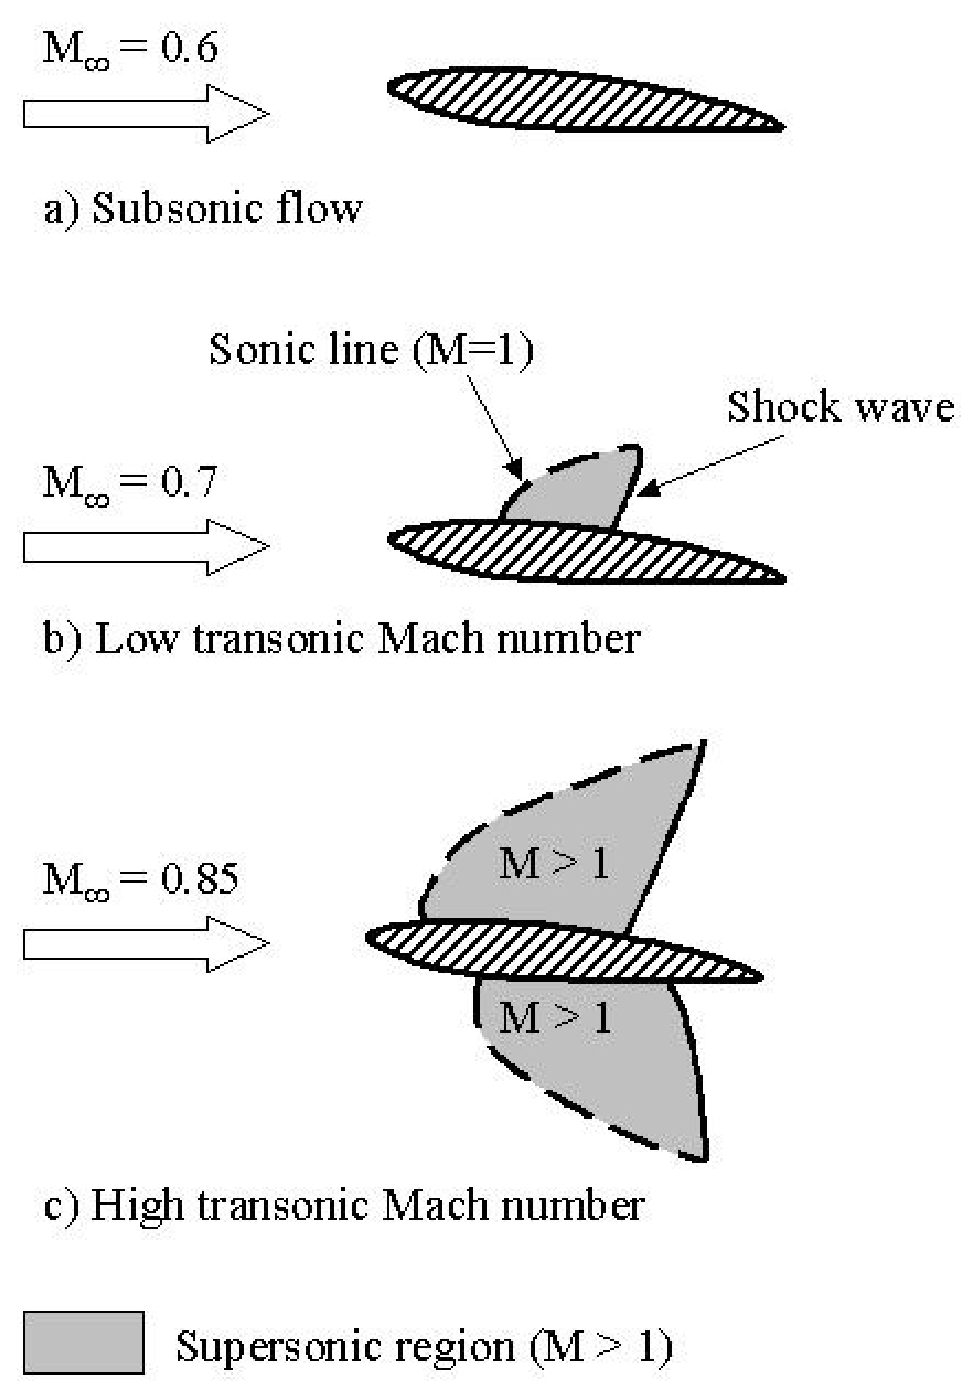
\includegraphics[height=6in]{aflow}
    \else
      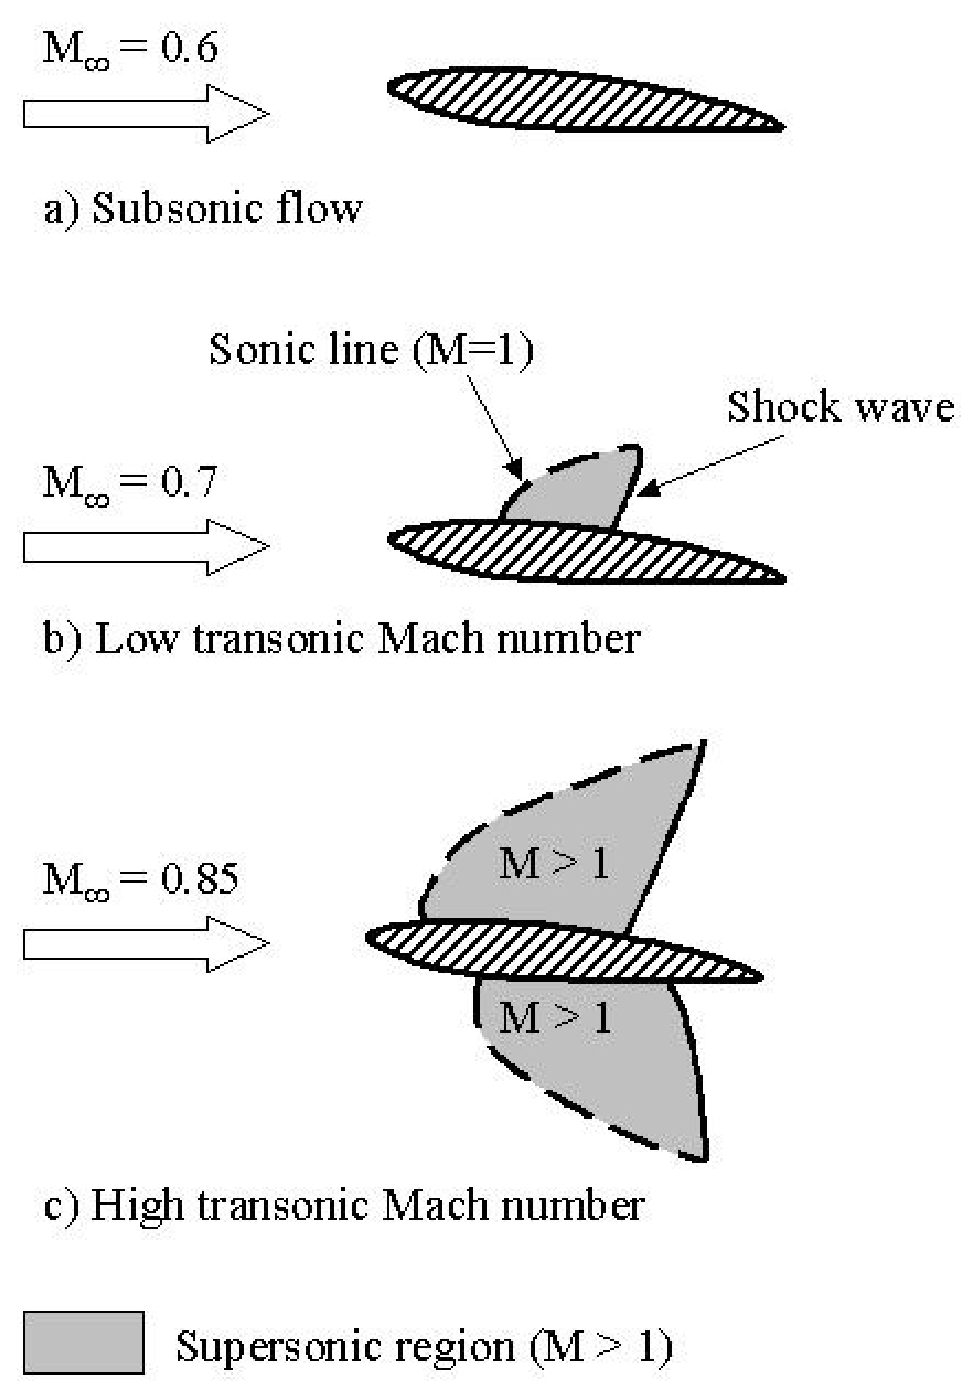
\includegraphics[bb = 92 86 545 742, height=6in]{aflow}
    \fi
    \caption{Airfoil Picture}
    \label{FigAir}
  \end{center}
\end{figure}

% above code has been macro-fied in Classes/MacroFile.tex file
%\InsertFig{\IncludeGraphicsH{aflow}{6in}{92 86 545 742}}{Airfoil Picture}{FigAir}

So as we have now labelled it we can reference it, like so (\ref{FigAir}) and it
is on Page \pageref{FigAir}. And as we can see, it is a very nice picture and we
can talk about it all we want and when we are tired we can move on to the next
chapter ...

I would also like to add an extra bookmark in acroread like so ...
\ifpdf
  \pdfbookmark[2]{bookmark text is here}{And this is what I want bookmarked}
\fi
% ------------------------------------------------------------------------


%%% Local Variables: 
%%% mode: latex
%%% TeX-master: "../thesis"
%%% End: 

\chapter{My Second Chapter}
\ifpdf
    \graphicspath{{Chapter2/Chapter2Figs/PNG/}{Chapter2/Chapter2Figs/PDF/}{Chapter2/Chapter2Figs/}}
\else
    \graphicspath{{Chapter2/Chapter2Figs/EPS/}{Chapter2/Chapter2Figs/}}
\fi

\section{First Section}
\markboth{\MakeUppercase{\thechapter. My Second Chapter }}
And now I begin my second chapter here ...

\section{Second Section}
\markboth{\MakeUppercase{\thechapter. My Second Chapter }}
and here I write more ...

\subsection{first subsection in the Second Section}
... and some more ...

\subsection{second subsection in the Second Section}
... and some more ...

\subsection{third subsection in the Second Section}
... and some more ...

% ------------------------------------------------------------------------

%%% Local Variables: 
%%% mode: latex
%%% TeX-master: "../thesis"
%%% End: 

\chapter{My Third Chapter}
\ifpdf
    \graphicspath{{Chapter3/Chapter3Figs/PNG/}{Chapter3/Chapter3Figs/PDF/}{Chapter3/Chapter3Figs/}}
\else
    \graphicspath{{Chapter3/Chapter3Figs/EPS/}{Chapter3/Chapter3Figs/}}
\fi

\section{First Section of the Third Chapter}
\markboth{\MakeUppercase{\thechapter. My Third Chapter }}{\thechapter. My Third Chapter}
And now I begin my third chapter here ...

\subsection{first subsection in the First Section}
... and some more 

\subsection{second subsection in the First Section}
... and some more ...

\subsubsection{first subsub section in the second subsection}
... and some more in the first subsub section otherwise it all looks the same
doesn't it? well we can add some text to it ...

\subsection{third subsection in the First Section}
... and some more ...

\subsubsection{first subsub section in the third subsection}
... and some more in the first subsub section otherwise it all looks the same
doesn't it? well we can add some text to it and some more and some more and
some more and some more and some more and some more and some more ...

\subsubsection{second subsub section in the third subsection}
... and some more in the first subsub section otherwise it all looks the same
doesn't it? well we can add some text to it ...

\section{Second Section of the Third Chapter}
\markboth{\MakeUppercase{\thechapter. My Third Chapter }}{\thechapter. My Third Chapter}
and here I write more ...

% ------------------------------------------------------------------------


%%% Local Variables: 
%%% mode: latex
%%% TeX-master: "../thesis"
%%% End: 

\def\baselinestretch{1}
\chapter{My Conclusions ...}
\ifpdf
    \graphicspath{{Conclusions/ConclusionsFigs/PNG/}{Conclusions/ConclusionsFigs/PDF/}{Conclusions/ConclusionsFigs/}}
\else
    \graphicspath{{Conclusions/ConclusionsFigs/EPS/}{Conclusions/ConclusionsFigs/}}
\fi

\def\baselinestretch{1.66}

Here I put my conclusions ...

%%% ----------------------------------------------------------------------

% ------------------------------------------------------------------------

%%% Local Variables: 
%%% mode: latex
%%% TeX-master: "../thesis"
%%% End: 


\backmatter % book mode only
\appendix
\chapter{Appdx A}

and here I put a bit of postamble ...

% ------------------------------------------------------------------------

%%% Local Variables: 
%%% mode: latex
%%% TeX-master: "../thesis"
%%% End: 

\chapter{Appdx B}

and here I put some more postamble ...

% ------------------------------------------------------------------------

%%% Local Variables: 
%%% mode: latex
%%% TeX-master: "../thesis"
%%% End: 


\bibliographystyle{plainnat}
%\bibliographystyle{Classes/CUEDbiblio}
%\bibliographystyle{Classes/jmb}
%\bibliographystyle{Classes/jmb} % bibliography style
\renewcommand{\bibname}{References} % changes default name Bibliography to References
\bibliography{References/references} % References file

\end{document}
